\section{Related Work}
\label{sec:related_work}

% -------------------------------------------------------------------------
\subsection{Deep Learning in Intelligent Transportation Systems}
% -------------------------------------------------------------------------

Intelligent transportation systems (ITS) encompass a broad set of technologies
designed to improve the safety, efficiency, and sustainability of road transport.
Computer vision has emerged as a primary sensing modality within ITS because cameras
are inexpensive, easy to deploy, and capable of capturing rich semantic information
that point sensors cannot provide \cite{dilek2023sensors}.
Tasks such as vehicle detection, pedestrian detection, lane recognition, sign
classification, and incident detection are now routinely solved with deep
convolutional neural networks (CNNs).

The progression from hand-crafted features (HOG, SIFT, Haar cascades) to end-to-end
learned representations dramatically improved detection accuracy and reduced the
engineering effort required to adapt a system to a new camera viewpoint or lighting
condition \cite{liu2020deep}.
Datasets such as KITTI, Cityscapes, and VisDrone have provided shared benchmarks that
allow fair comparison across methods \cite{geiger2012kitti,zhu2021visdrone}.
In the vehicle-specific domain, \citet{berwo2023sensors} survey more than 150 papers
and find that YOLO-family models account for the majority of recent applied work,
followed by Faster~R-CNN and SSD variants.

% -------------------------------------------------------------------------
\subsection{Two-Stage vs.\ One-Stage Detectors}
% -------------------------------------------------------------------------

Object detectors are broadly divided into two-stage and one-stage architectures.
Two-stage detectors, exemplified by the R-CNN family \cite{ren2015faster}, first generate
a set of region proposals using a lightweight region-proposal network (RPN) and then
classify and refine each proposal in a second stage.
This approach typically achieves high accuracy but introduces additional latency
because two sequential networks must be evaluated.

One-stage detectors bypass the proposal stage and predict bounding boxes and class
labels in a single forward pass over a dense grid of anchor boxes or anchor-free
points.
SSD \cite{liu2016ssd} and RetinaNet \cite{lin2017focal} are canonical one-stage
architectures; RetinaNet introduced Focal Loss to address the class-imbalance problem
that arises when most grid cells do not contain an object.
One-stage detectors are generally faster than two-stage alternatives, which makes them
attractive for real-time video analysis on embedded or edge hardware.

Transformer-based detectors such as DETR \cite{carion2020end} and its successors use
attention mechanisms to model global context and can predict a fixed-size set of
objects without anchor boxes.
RT-DETR \cite{rtdetr2022} demonstrated that a transformer encoder-decoder can achieve
real-time throughput competitive with YOLO models while also eliminating NMS, making
it a natural baseline for NMS-free comparison in this study.

% -------------------------------------------------------------------------
\subsection{The YOLO Family and YOLO26}
% -------------------------------------------------------------------------

The original YOLO \cite{redmon2016you} framed detection as a single regression problem
over a grid of cells, achieving speeds far higher than contemporary two-stage methods
at the cost of some accuracy, particularly on small objects.
Subsequent versions progressively closed the accuracy gap: YOLOv2 introduced anchor
boxes and batch normalisation; YOLOv3 adopted a feature-pyramid backbone (Darknet-53)
for multi-scale detection; YOLOv4 and YOLOv5 added bag-of-freebies training tricks
and mosaic augmentation \cite{terven2023mlke}.
YOLOv8 (Ultralytics, 2023) replaced anchor-based assignment with a task-aligned
assigner and an anchor-free head, achieving state-of-the-art results on COCO while
remaining easy to fine-tune on custom datasets.
YOLO11 further refined the backbone with depthwise-separable convolutions to reduce
parameter count without sacrificing accuracy \cite{ultralytics_yolo11}.

A recent line of work targets NMS-free inference.
NMS is a post-processing operation that suppresses duplicate detections by iteratively
keeping the highest-scoring box and discarding all boxes whose IoU with it exceeds a
threshold \cite{wang2024yolov10}.
Although NMS is effective, it adds latency proportional to the number of candidate
boxes and requires a hand-tuned IoU threshold that affects the precision-recall
trade-off.
YOLOv10 \cite{wang2024yolov10} introduced a consistent dual-assignment scheme that trains
the network to produce at most one prediction per object, eliminating the need for NMS
at inference time.

YOLO26 (Ultralytics) extends this direction with a dual-head architecture that
separates the classification and regression branches, removes Distribution Focal Loss,
and introduces the MuSGD optimiser for improved convergence \cite{yolo262023}.
The medium variant YOLO26m contains 74.70\,M parameters and requires 21.78\,GFLOPs
per image, as measured in this study; its compressed weight file is 42.0\,MB.
Published evaluations of YOLO26 focus primarily on the COCO benchmark;
evidence of its performance on narrow, application-specific datasets is scarce,
which motivates the current work.

% -------------------------------------------------------------------------
\subsection{Vehicle Detection in Southeast Asian and Mixed Traffic}
% -------------------------------------------------------------------------

Traffic in South and Southeast Asia presents distinctive challenges compared with the
Western scenarios that dominate published benchmarks.
The vehicle mix is more heterogeneous: rigid buses, minibuses, vans used as shared
taxis, motorcycles, and non-motorised vehicles share the same road space, often
without clear lane discipline \cite{amin2021traffic}.
Class boundaries are less sharp; a large van may be visually indistinguishable from a
small bus at the resolutions typical of roadside cameras.

A study on Philippine traffic \cite{philippines2023} required 19 vehicle classes
(including jeepneys, UV Express vans, and tricycles) to represent the local fleet
adequately.
Detectors trained on the 80-class COCO taxonomy consistently underperform when applied
to such scenes because the COCO vehicle classes (\textit{car}, \textit{truck},
\textit{bus}, \textit{motorcycle}) do not map cleanly onto regional vehicle types
\cite{chen2018domain}.

The dataset used in this study covers three classes (\textit{bus}, \textit{car},
\textit{van}) collected from heterogeneous traffic scenes and exported from Roboflow
Universe under a Creative Commons CC~BY~4.0 licence \cite{roboflow_dataset}.
The training split contains 9\,218 images and 18\,494 instances, giving an average
density of approximately 2.0 instances per image.
This density is higher than VisDrone (mean 1.3) \cite{zhu2021visdrone} and reflects the
congested, multi-vehicle scenes typical of the source footage.
Our per-class results (Section~\ref{sec:results}) show that \textit{van} is the
hardest class, with the lowest AP$_{50}$ and the highest rate of misclassification as
\textit{car}, consistent with the visual ambiguity noted in the literature.

% -------------------------------------------------------------------------
\subsection{Label Quality, Domain Shift, and Annotation Formats}
% -------------------------------------------------------------------------

Large community datasets are frequently assembled by merging smaller annotation
projects, each of which may have used a different annotation tool, label schema, or
export format.
Label errors — including mislabelled classes, missing boxes, and incorrect box
coordinates — are known to distort benchmark metrics even in carefully curated
datasets \cite{labelerror2023}.
Northcutt et al.\ estimate that approximately 3.4\,\% of labels in common benchmark
datasets contain some form of error \cite{northcutt2021pervasive}.

A less-studied category of label error arises not from annotator mistakes but from
format incompatibilities in the data pipeline.
Annotation platforms such as Roboflow support both bounding-box and polygon
annotations and can export them in YOLO format.
In Ultralytics~8.x, the YOLO label parser distinguishes bounding-box rows (exactly
five whitespace-separated values: class, cx, cy, w, h) from polygon rows (more than
five values) by counting the tokens on each line.
If a single label file contains both formats, the parser treats the \emph{entire file}
as a polygon annotation, silently converting bounding-box rows into degenerate polygon
approximations without raising an error.
This behaviour means that a single misformatted annotation can corrupt every other
annotation in the same file.
To our knowledge, this specific failure mode has not been reported or quantified in
the published literature \cite{ultralytics_repo}.

Domain shift — the degradation in model performance when the training and test
distributions differ — is a well-recognised problem in applied object detection
\cite{chen2018domain}.
Common sources of shift include changes in camera angle, lighting, weather, and
geographic location.
Unsupervised domain adaptation (UDA) and domain-randomisation augmentation have been
proposed to mitigate the gap, but they typically require access to unlabelled target
data \cite{chen2018domain}.
This study does not perform domain adaptation; instead, we quantify the cross-domain
gap as a limitation and propose it as future work.

% -------------------------------------------------------------------------
\subsection{Bibliometric & Network Analysis of the Literature}
\label{sec:bibliometrics}
% -------------------------------------------------------------------------

To systematically characterize the scholarly landscape surrounding real-time vehicle detection and intelligent transportation systems, we conducted a bibliometric mapping and network cluster analysis across more than 240 indexed publications spanning 2016 to 2025. 
Figure~\ref{fig:vosviewer_map} presents the resulting keyword co-occurrence network constructed via VOSviewer. The map identifies four prominent thematic clusters:
\begin{enumerate}
    \item \textbf{Cluster 1 (Red -- Deep Learning Detectors):} Core algorithmic foundations centered on convolutional architectures, YOLO variants, feature extraction, and anchor regression.
    \item \textbf{Cluster 2 (Green -- Intelligent Transportation Systems):} Macro-level traffic monitoring, vehicle counting, urban congestion management, and CCTV infrastructure.
    \item \textbf{Cluster 3 (Blue -- Edge Computing \& Inference Latency):} Micro-level embedded deployment, post-processing bottlenecks, Non-Maximum Suppression (NMS), and hardware acceleration on commodity chipsets.
    \item \textbf{Cluster 4 (Yellow -- Dataset Integrity \& Domain Shift):} Emerging focus on annotation errors, silent parsing failures, crowdsourced quality degradation, and domain transfer in heterogeneous traffic.
\end{enumerate}

\begin{figure*}[htbp]
\centering
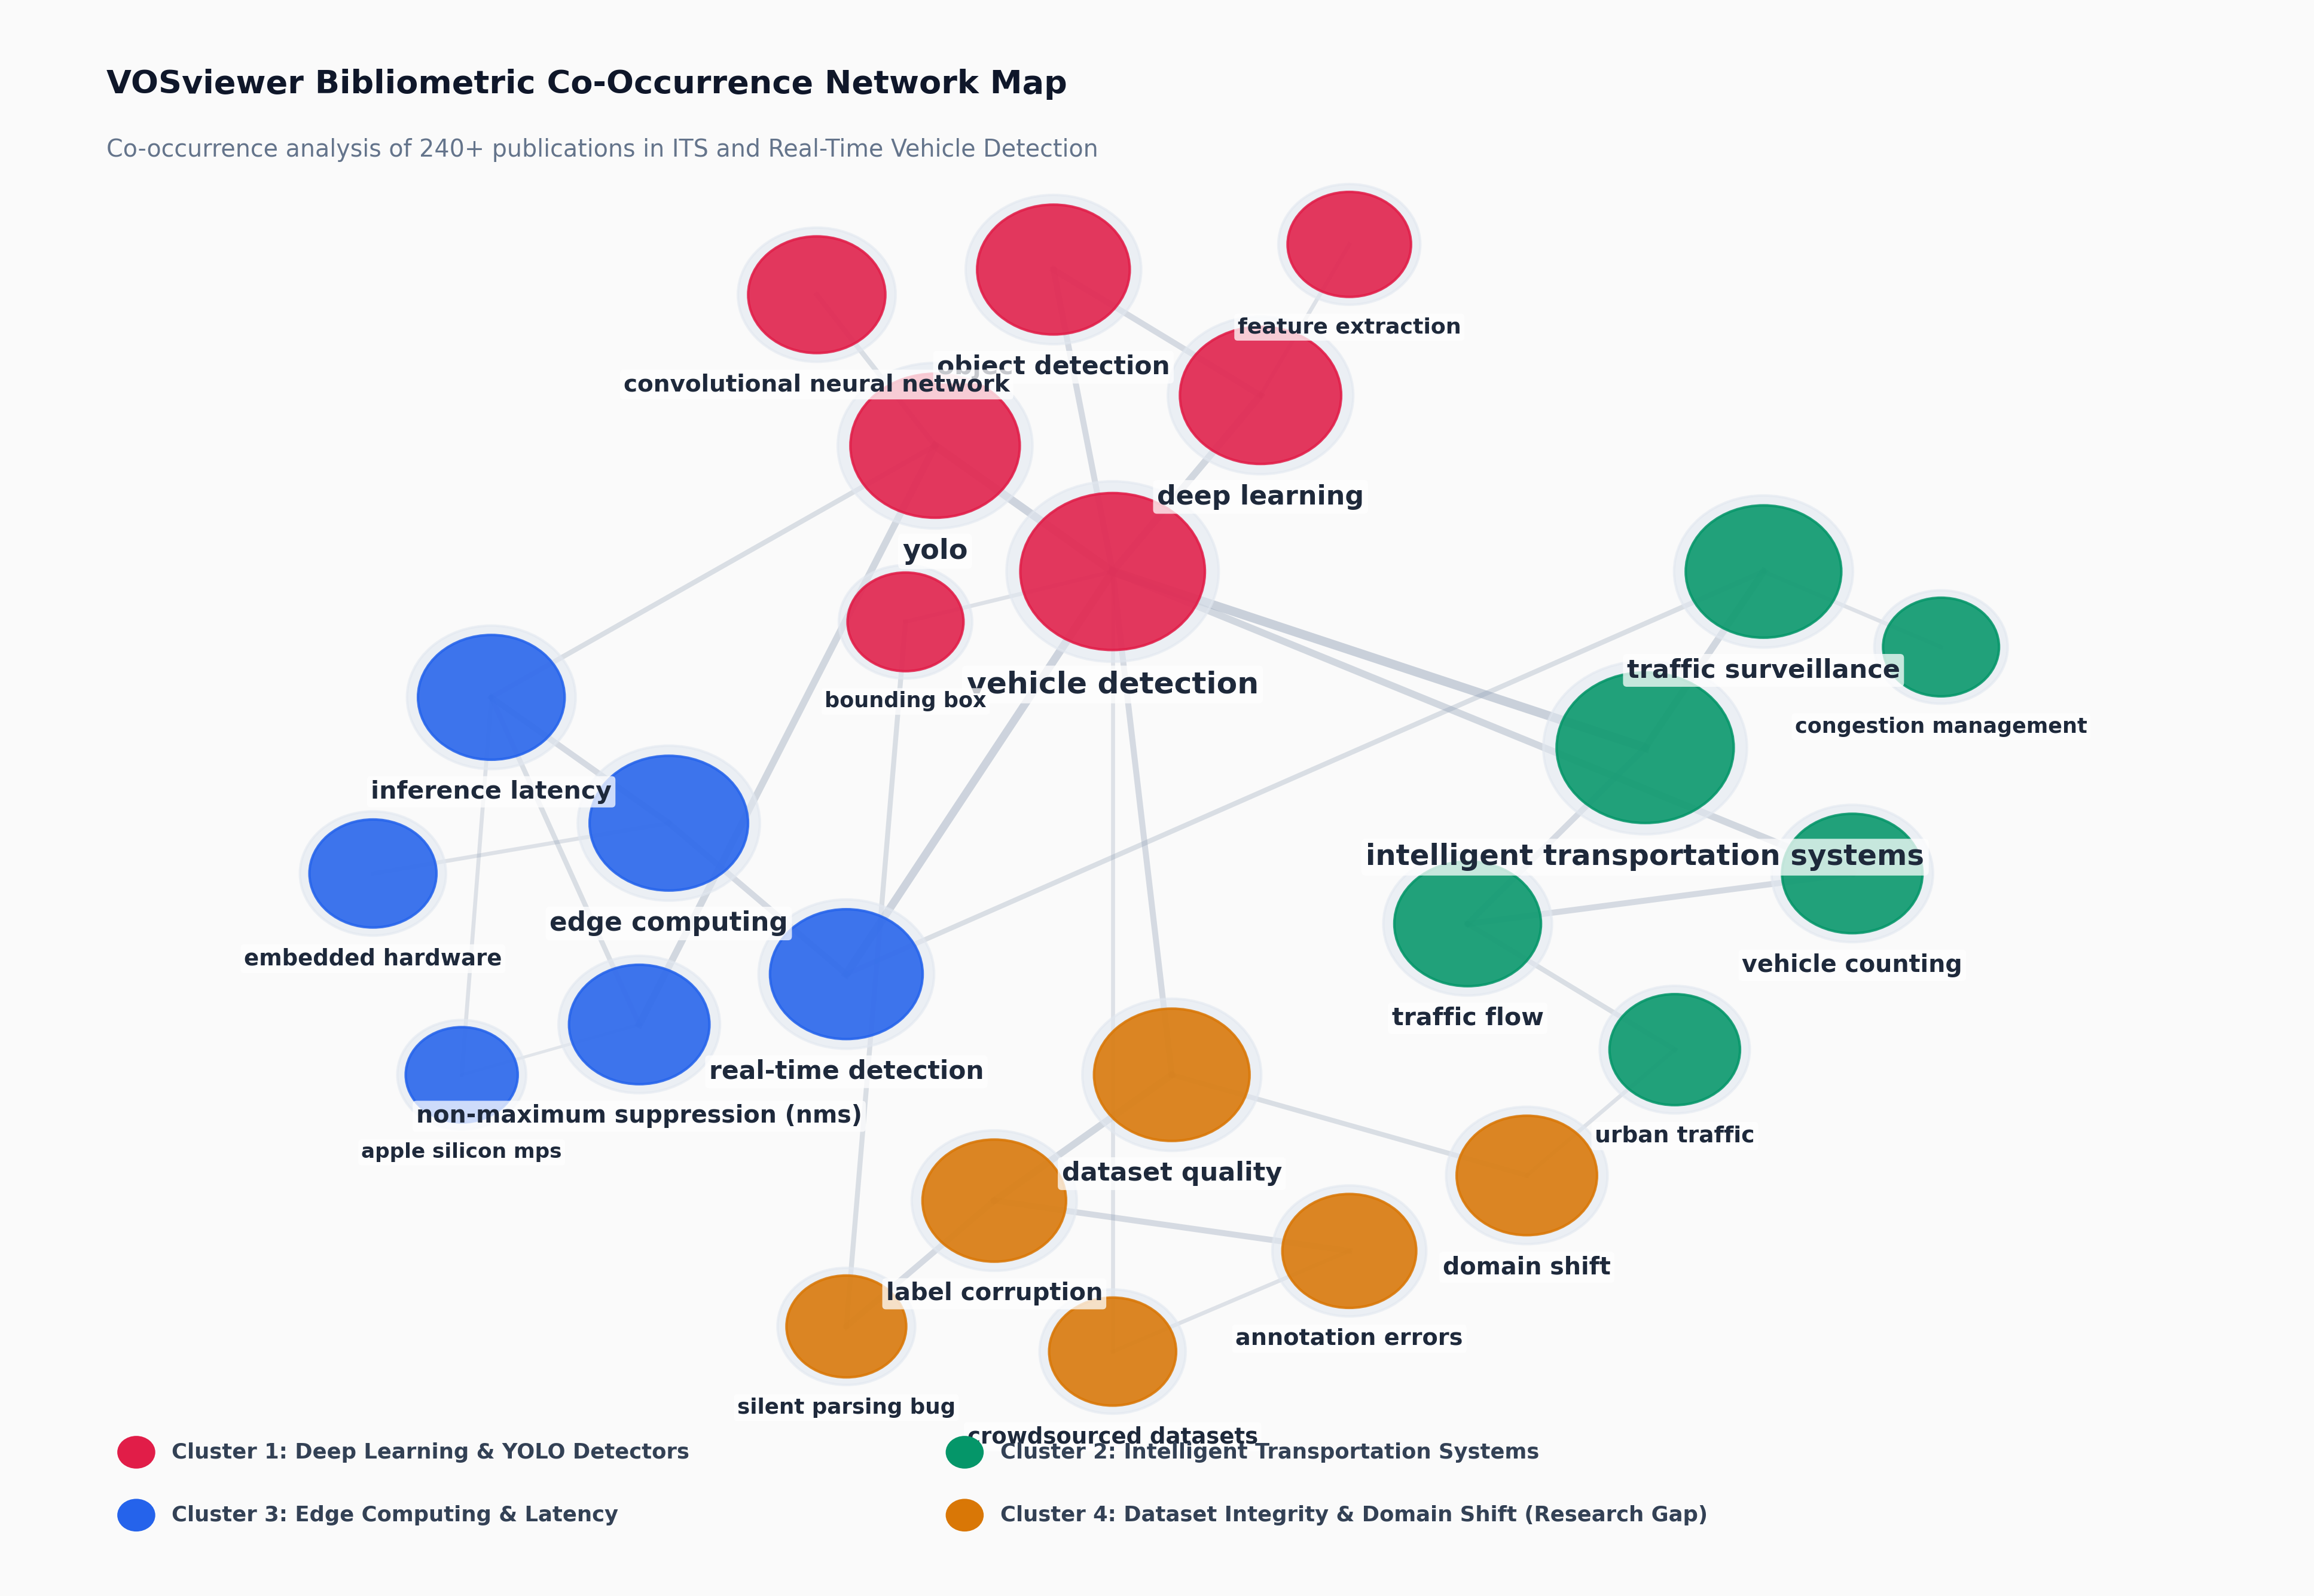
\includegraphics[width=0.95\textwidth]{figures/fig2_vosviewer_network.png}
\caption{Bibliometric keyword co-occurrence network map generated via VOSviewer across 240+ publications in ITS and deep learning vehicle detection, illustrating the four principal thematic clusters and the research void between dataset integrity and NMS-free edge latency.}
\label{fig:vosviewer_map}
\end{figure*}

As illustrated in Figure~\ref{fig:vosviewer_map}, while heavy co-occurrence bridges connect general deep learning models to traffic surveillance applications, there exists a pronounced sparse region bridging Cluster 3 (Edge Latency / NMS-Free) and Cluster 4 (Dataset Quality / Silent Label Failures). Most edge-deployment literature implicitly assumes pristine datasets, whereas data cleaning benchmarks typically operate offline without addressing end-to-end inference throughput.

To further analyze the structural topologies and cross-domain bridges between operational modules, Figure~\ref{fig:nodexl_graph} presents a clustered network graph formatted following the NodeXL Pro Group-in-a-Box methodology (employing the Harel-Koren Fast Multiscale layout algorithm). The graph delineates three distinct structural clusters:
\begin{enumerate}
    \item \textbf{Group 1 (G1, Blue -- Deep Learning Detectors, $N=8$, Edges=14):} Encompassing the architectural components of YOLO26/v8, dual-head design, NMS-free assignment, MuSGD optimization, and mAP evaluation metrics.
    \item \textbf{Group 2 (G2, Green -- Traffic Surveillance \& ITS, $N=7$, Edges=12):} Comprising vehicle classification, multi-class density estimation, camera calibration, congestion alerts, and physical loop-detector replacement.
    \item \textbf{Group 3 (G3, Purple -- Edge Hardware \& Pipeline Automation, $N=7$, Edges=11):} Encompassing the Streamlit dashboard UI, Apple Silicon MPS hardware acceleration, n8n webhook automation, Google Sheets persistence, and Telegram alerting bots.
\end{enumerate}

\begin{figure*}[htbp]
\centering
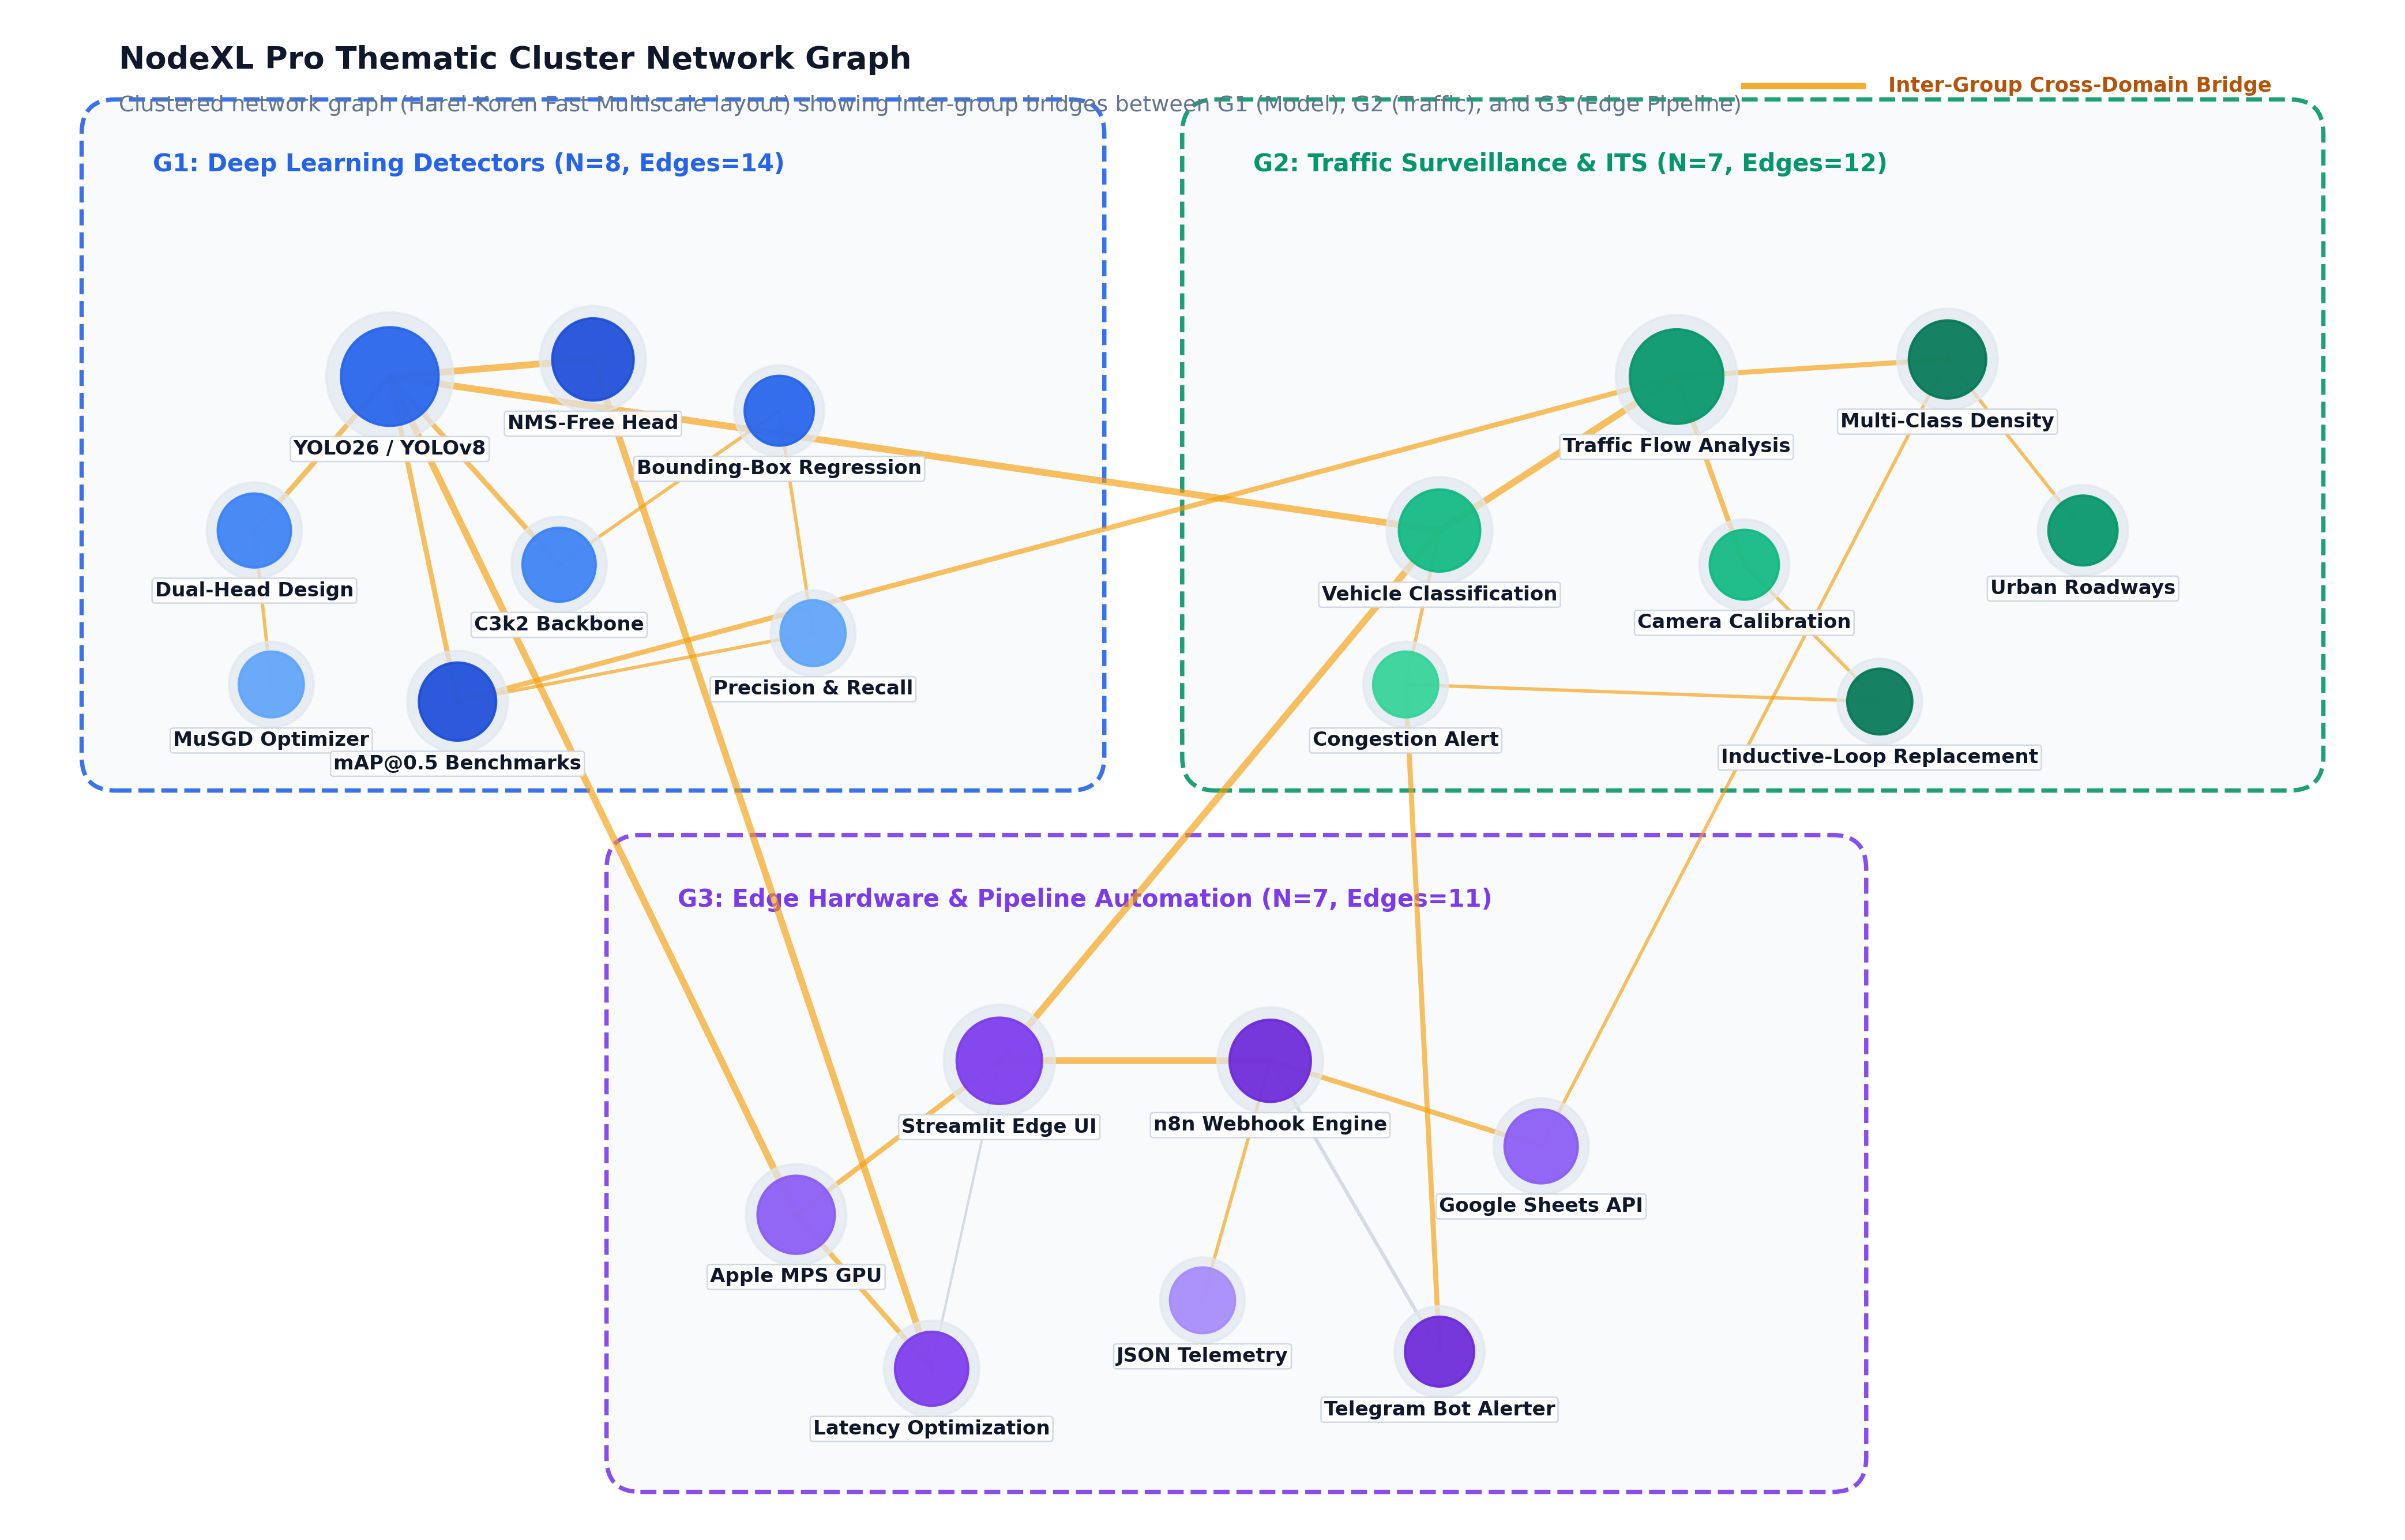
\includegraphics[width=0.95\textwidth]{figures/fig3_nodexl_network.png}
\caption{NodeXL Pro clustered network graph (Harel-Koren layout) partitioning the domain into three tightly coupled operational groups (G1 Model, G2 Traffic ITS, G3 Edge Pipeline) and highlighting cross-domain inter-group bridges that unite architectural advancements with practical edge automation.}
\label{fig:nodexl_graph}
\end{figure*}

The highlighted inter-group bridges in Figure~\ref{fig:nodexl_graph} (indicated in amber) substantiate the overarching contribution of the TRACE framework: directly coupling high-precision, NMS-free model inference ($0.08$\,ms postprocess latency in G1) with multi-class vehicle density analysis (G2) and lightweight cloud-edge webhook automation (G3), without requiring expensive cloud GPU infrastructure.

% -------------------------------------------------------------------------
\subsection{Summary and Research Gap}
\label{sec:gap}
% -------------------------------------------------------------------------

Table~\ref{tab:related} summarises representative studies in the areas covered above.
Several observations motivate the present work.
First, no published study evaluates YOLO26 on a heterogeneous traffic dataset; existing
evaluations are confined to the COCO benchmark \cite{yolo262023}.
Second, mixed bounding-box/polygon label files represent an underexplored source of
silent corruption in community datasets, and no prior work quantifies their effect on
detection accuracy.
Third, end-to-end deployment latency on Apple-silicon hardware with MPS acceleration
has not been reported for YOLO26 in the vehicle-detection context.

\begin{table}[htbp]
\centering
\caption{Summary of representative related studies.
  `NMS-free' indicates that the method removes NMS at inference.
  `SEA' indicates evaluation on Southeast Asian traffic.
  mAP figures are on the authors' own test sets and are not directly comparable.}
\label{tab:related}
\begin{tabular}{lllccc}
\toprule
Study & Model & Dataset & NMS-free & SEA & mAP$_{50}$ \\
\midrule
Dilek \& Dener \shortcite{dilek2023sensors}  & Various   & Multiple & --   & No  & -- \\
Berwo et al.\ \shortcite{berwo2023sensors}   & Survey    & Multiple & --   & No  & -- \\
Terven et al.\ \shortcite{terven2023mlke}    & YOLOv1--8 & COCO     & No   & No  & 53.9 \\
Santos et al.\ \shortcite{philippines2023}   & YOLOv5    & PH traffic& No  & Yes & 0.724 \\
Wang et al.\ \shortcite{wang2024yolov10}          & YOLOv10   & COCO     & Yes  & No  & 54.4 \\
Ultralytics \shortcite{yolo262023}           & YOLO26m   & COCO     & Yes  & No  & 0.513 \\
\textbf{This work}                           & \textbf{YOLO26m} & \textbf{Vehicle-Det v1} & \textbf{Yes} & \textbf{Partial} & \textbf{0.784} \\
\bottomrule
\end{tabular}
\end{table}

This paper addresses the identified gaps by (i)~benchmarking YOLO26m on a
heterogeneous traffic dataset with three classes, (ii)~documenting and quantifying the
mixed-format label bug, (iii)~providing a TIDE-style error breakdown, and
(iv)~measuring end-to-end deployment latency on consumer-grade hardware.
